\documentclass[11pt]{article}

% Language setting 
\usepackage[spanish]{babel}

% Set page size and margins
\usepackage[a4paper,top=2cm,bottom=2cm,left=2.7cm,right=2.7cm,marginparwidth=1.75cm]{geometry}
\setlength
\parindent{0pt}

% Useful packages 
\usepackage{amsmath} 
\usepackage{graphicx}
\usepackage[colorlinks=true, linkcolor=black, urlcolor=blue]{hyperref}

% Uncomment these packages if you want to use dark mode % \usepackage{darkmode}
% \enabledarkmode

\usepackage{listings}
\usepackage{tcolorbox}
\usepackage{blindtext}  % For dummy text

\lstset{
    keywordstyle=\color{blue}\bfseries,
    basicstyle=\ttfamily\fontsize{10pt}{\baselineskip}\selectfont,
}



% Title and author 
\title{Tarea: Automatización de Software en el entorno MVF}
\author{Álvaro Hernández} 
\date{\today}

\begin{document}

%%%%%%%%%%%%%%%%%%%%%%%%%%%%%%%%%%

\maketitle 
\tableofcontents 
\newpage

\section*{Introducción}

En este trabajo se realizará una automatización de la configuración de una red de routers Cisco que se proporciona en el enuciado.
Para ello, se utilizará el software GNS3 para inizialicar y simular la red, y a ésta se aplicarán técnicas y configuraciones de automatización, monitorización, y gestión de red. 
El software que se usará para las distintas tareas será:

\begin{itemize}
    \item \textbf{Simulación}: Para la simulación, como se ha comentado antes, se usará GNS3 a partir de la topología proporcionada.
    \item \textbf{Automatización}: Aunque se haya mencionado el posible uso de scripts de Python en el enunciado, se usará Ansible para todas las tareas de automatización posibles, se intentará mantener todo en el mismo \textbf{archivo yaml}
    \item \textbf{Monitorización}: Se usará el \textbf{protocolo SNMP} para la monitorización de la red, con software como Cacti, OpenObserver o MIB Browser.
\end{itemize}

\section{Implementación / Configuración de la topología}

El primer ejercicio trata sobre la implementación de la topología proporcionada por el mismo. Se realiza el diseño mediante GNS3, sin configurar nada más que añadir las conexiones de todos los elementos. Tras esto, la topología queda de la siguiente manera:


\begin{figure}[h]
    \centering
    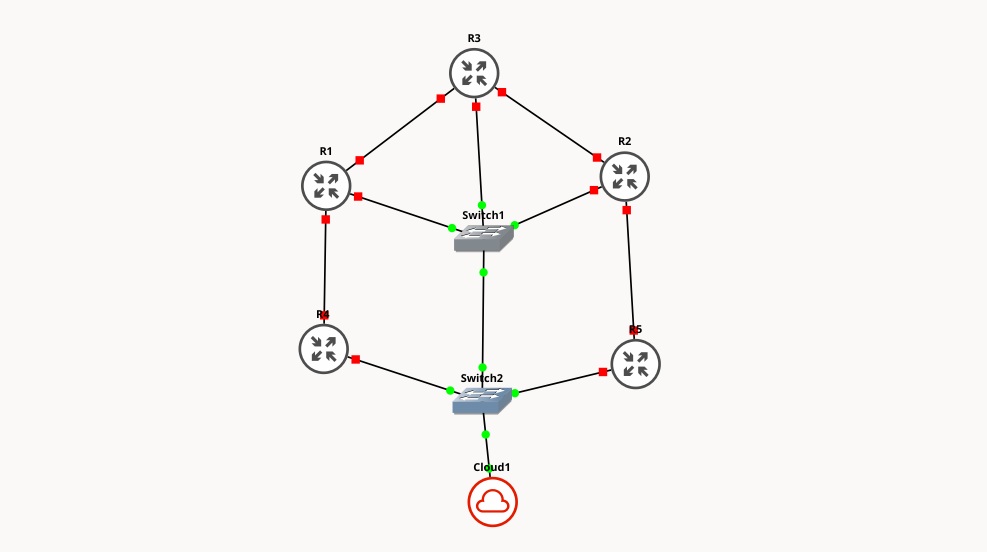
\includegraphics[width=\textwidth]{src/topologia.png}
    \caption{Topología de la red}
\end{figure}

No se ha configurado ni hostnames ni interfaces para dejarle el trabajo a Ansible.

Para iniciar con la configuración, que se hará mediante Ansible, hará falta configurar ssh para la conexión de forma segura, y una ip de interfaz para poder realizar la conexión. Por lo que mediante GNS3 se configurará lo mínimo necesario para este funcionamiento. Esta configuración será la proporcionada en \href{https://github.com/plopezmp/GdR}{el Github de configuración de Ansible de la asignatura}, adaptando las IPs e interfaces a nuestra topología. Un ejemplo con el MU-NN sería el siguiente (desde la configuración del router ya):

\begin{tcolorbox}[
    boxrule=0pt,
]
    \begin{lstlisting}[gobble=6]
        int g0/0 
        ip address 172.18.0.220 255.255.255.0
        exit
        line vty 0 15
        login local
        transport input all
        exit 
        enable secret cisco 
        line console 0 
        passw cisco
        login 
        exit 
        ip domain-name upct 
        username ansible privilege 15 secret ansible
        ip ssh time-out 60
        crypto key generate rsa usage-keys label router-key
        # Y seleccionamos 1024 bits para ambas opciones.
    \end{lstlisting}
\end{tcolorbox}

Con esto se podría realizar la conexión con ssh, por lo que Ansible se podrá conectar. Comprobamos que se puede conectar a ssh con el usuario ansible y la contraseña ansible.

\begin{figure}[h]
    \centering
    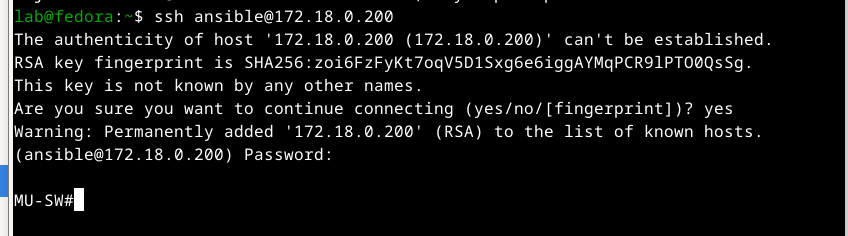
\includegraphics[width=\textwidth]{src/ssh.png}
    \caption{Conexión ssh con el router MU-Sw}
\end{figure}

Una vez comprobado que todos los routers se pueden conectar mediante ssh, se procede a la configuración de Ansible. Se pide configurar el resto de las interfaces junto al loopback y hostnames. 

Para iniciar con la configuración, se creará un archivo \texttt{hosts} con los routers que se quieren configurar, y se reciclará el archivo \texttt{ansible.cfg} del repositorio de la asignatura para que Ansible no pida confirmación para las conexiones ssh. El archivo hosts está accesible en la entrega del trabajo. 

Para las \textbf{plays} de Ansible, se ha creado un archivo \texttt{tarea.yml} que recoge todas las acciones que hará ansible en un único archivo. Cada router tendrá una play, por lo que nuestra \texttt{tarea.yml} tendrá este formato:

\begin{tcolorbox}[
    boxrule=0pt,
    title=Formato que seguirá tarea.yml,
]
    \begin{lstlisting}[gobble=6]
        ---
        - name: Configure interface g1/0 on the router 
        hosts: R1
        gather_facts: no 
        connection: network_cli 
        tasks:
            - name: Configure router...
            ios_command:
                commands:
                    - interface GigabitEthernet1/0
                    - ... 
                register: output

    \end{lstlisting}
\end{tcolorbox}

Una vez terminado el archivo \texttt{tarea.yml}, cuyo contenido del script se puede comprobar en la entrega del trabajo, cada router tendrá la configuración de sus interfaces respectivas, se ejecutará de la siguiente forma para que se realicen las configuraciones:

\begin{tcolorbox}[
    boxrule=0pt,
    title=Script de ejecución de Ansible,
]
    \begin{lstlisting}[language=bash, gobble=6]
        #! /bin/bash
        workon ansible
        ansible-playbook -i hosts tarea.yml
        #-i para indicar los inputs que seran hosts y tarea.yml
    \end{lstlisting}
\end{tcolorbox}

Si la ejecución es correcta, tendremos el siguiente output de Ansible que nos indica que no han habido errores:

\begin{figure}[h]
    \centering
    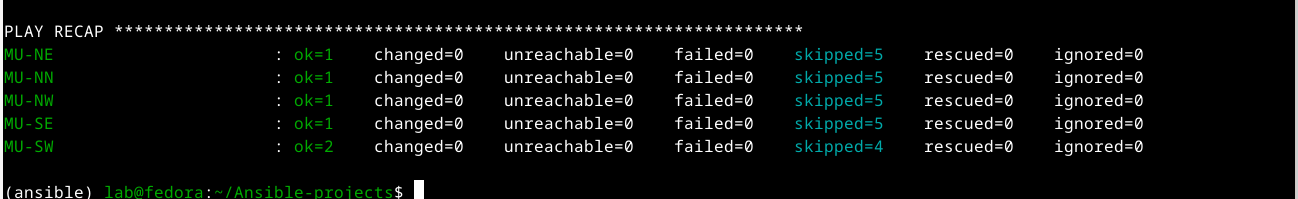
\includegraphics[width=\textwidth]{src/ansible.png}
    \caption{Output de Ansible tras la ejecución}
\end{figure}



\section{Encaminamiento}

En este ejercicio se pide configurar el encaminamiento de la red. Para ello, se continuará el archivo \texttt{tarea.yml} ya que se se considera igualmente como configuración inicial. Se añade a la tarea de \textbf{Ansible} el protocolo de encaminamiento OSPF, anunciando las redes correspondientes a cada interfaz del router. El formato de la configuración de OSPF será el siguiente (ejemplo para MU-NN)

\begin{tcolorbox}[
    boxrule=0pt,
    title=Configuración de OSPF en MU-NN, 
]
    \begin{lstlisting}[gobble=6]
          - router ospf 1
          - network 172.18.0.0 0.0.0.255 area 0
          - network 22.10.0.0 0.0.0.3 area 0
          - network 20.20.20.20 0.0.0.0 area 0
          - exit
          - wr
    \end{lstlisting}
\end{tcolorbox}

Se puede ver las configuraciones en \texttt{tarea.yml.} Para comprobar, haremos dos peticiones: una desde \texttt{MU-NN} a \texttt{MU-SE} y otra desde \texttt{MU-SE} a \texttt{MU-NN} 

\begin{figure}[h]
    \centering
    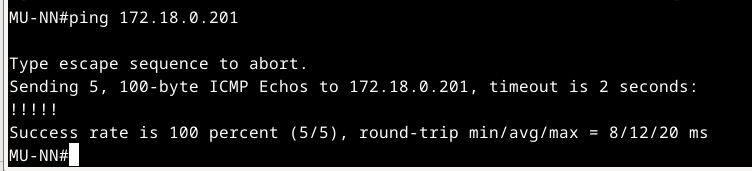
\includegraphics[width=\textwidth]{src/ping1.png}
    \caption{Ping de MU-NN a MU-SE }
\end{figure}


\begin{figure}[h]
    \centering
    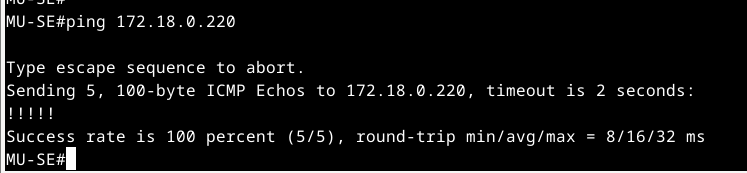
\includegraphics[width=\textwidth]{src/ping2.png}
    \caption{Ping de MU-SE a MU-NN }
\end{figure}


Con esto se puede ver que hay conectividad entre los routers, pero no se comprueba la implementación del protocolo OSPF al completo. Para ello, añadiremos una captura del router \texttt{MU-NN} con el comando \texttt{show ip ospf neighbor} para observar los vecinos OSPF.


\begin{figure}[h]
    \centering
    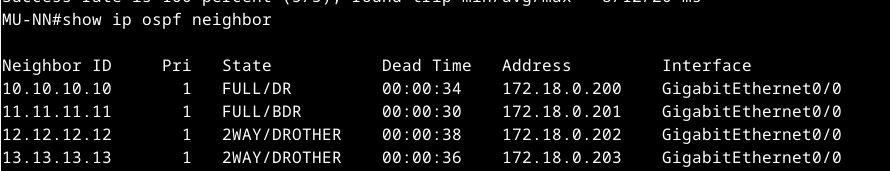
\includegraphics[width=\textwidth]{src/neighbors.png}
    \caption{Ping de MU-SE a MU-NN }
\end{figure}

Por lo que se habrá configurado OSPF correctamente.

\section{Activación de la gestión SNMP de los routers}

Para la activación de la gestión SNMP, se seguirá la práctica correspondiente que se dió en clase sobre el protocolo. Se configurarán los routers con valores y comandos similares. Por el momento, para activar SNMP se hará en el archivo \texttt{snmp.yml}:

\begin{tcolorbox}[
    boxrule=0pt,
    title=Configuración de OSPF en MU-NN, 
]
    \begin{lstlisting}[gobble=6]
          - snmp-server community AHR RW
          - snmp-server ifindex persist
    \end{lstlisting}
\end{tcolorbox}

Tras esto, se comprobará si está activo mediante SNMPGET desde MIB Browser. En la tabla de resultados se verá el objeto \texttt{sysDescr.O} del primer loopback que se hizo el snmpget, y el del segundo.

\begin{figure}[h]
    \centering
    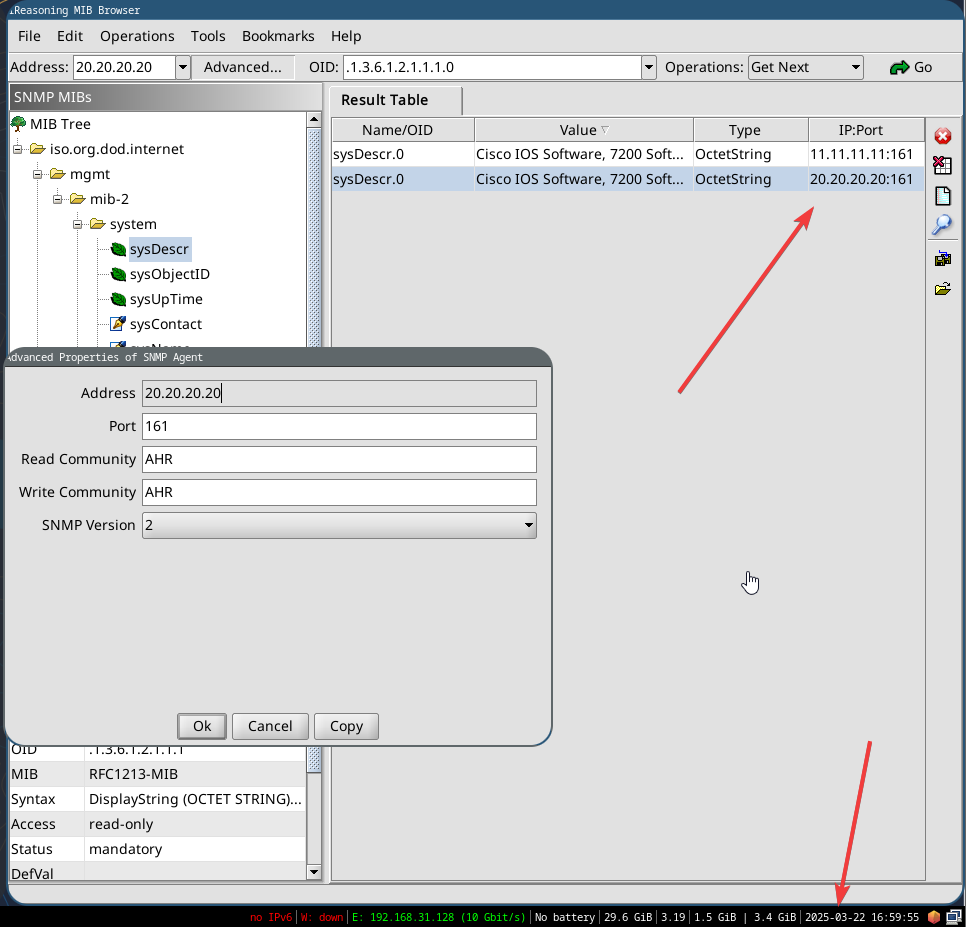
\includegraphics[width=\textwidth]{src/snmpgets.png}
    \caption{Comprobación de SNMP mediante MIB Browser}
\end{figure}

Una vez vemos que funciona correctamente, se activan los \texttt{traps}, \texttt{syslogs}, \mbox{\texttt{linkdown}}, \mbox{\texttt{linkup}}, \mbox{\texttt{coldstart}}, y \mbox{\texttt{warmstart}}. También, para el siguiente apartado, añadimos el servidor HTTP. Como todo viene en la misma sección, seguirá estando en el mismo archivo. Finalmente, en \texttt{snmp.yml} el formato de los routers será el siguiente:

\begin{tcolorbox}[
    boxrule=0pt,
    title= traps syslog y HTTP en el archivo snmp.yml, 
]
    \begin{lstlisting}[gobble=10]
          - configure terminal
          - snmp-server community AHR RW
          - snmp-server ifindex persist
          - snmp-server trap-source Loopback0
          - snmp-server enable traps snmp linkdown linkup coldstart warmstart
          - snmp-server enable traps bgp
          - snmp-server host 172.18.0.1 version 2c AHR 
          - logging facility local3
          - logging source-interface Loopback0
          - logging 172.18.0.5
          - ip http server
          - ip http authentication local
          - exit
          - wr
    \end{lstlisting}
\end{tcolorbox}

Para acceder al servidor HTTP, desde Firefox se accede a la ip del loopback que se ha configurado.

\begin{figure}[h]
    \centering
    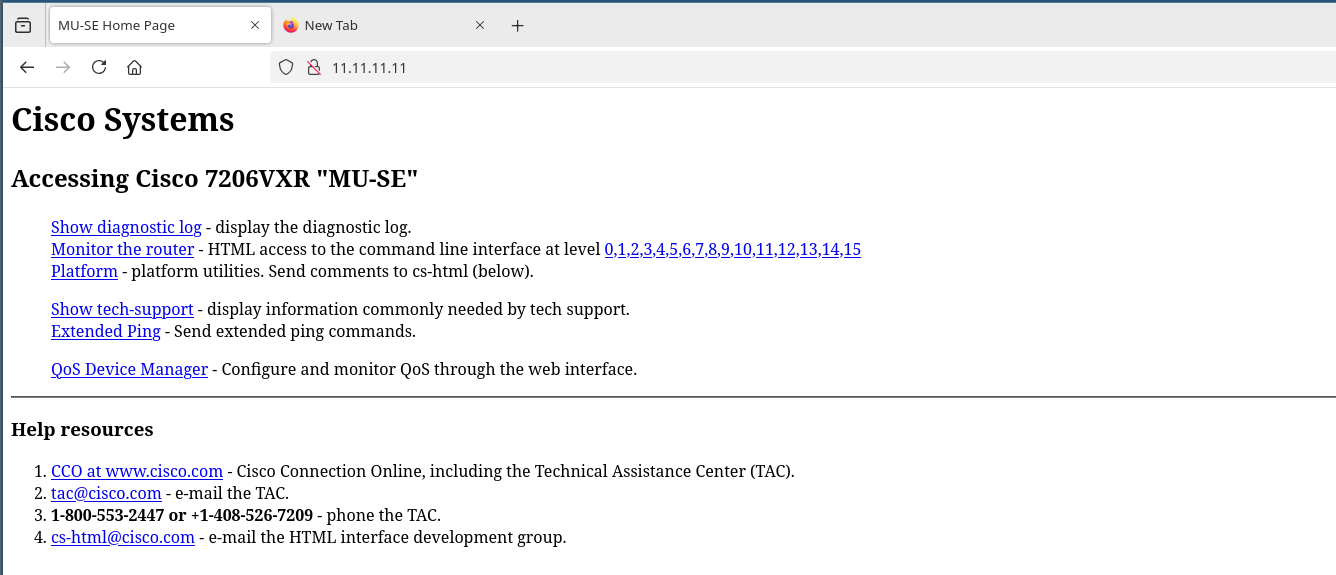
\includegraphics[width=\textwidth]{src/http.png}
    \caption{Acceso al servidor HTTP}
\end{figure}


\section{Configuración de Alarmas}

\subsection{Alarma 1: MU-NE}

Se configura la alarma en el router MU-NE, donde se añadirá el objeto correspondiente a la interfaz de entrada de la red. En la práctica hemos trabajado con el objeto \texttt{ifEntry}, y dentro de éste, el objeto \texttt{ifOutUcastPkts}. Este objeto funcionaría ya que debido a la respuesta, podría analizar el incremento del tráfico, pero en el enunciado se nos pide \textbf{paquetes de entrada}, por lo que, en vez de usar \texttt{ifOutUcastPkts}, se usará \texttt{ifInUcastPkts}. \textbf{La razón de usar} esta alarma es que, cumple con el funcionamiento que se pide, cumple el hecho de ser \textbf{tráfico de entrada}, y además, viene del objeto \texttt{ifEntry}, por lo que sabemos lo configurable que es y los valores con los que debemos trabajar.

El comando de la práctica pasa de \texttt{ifEntry.17.1 \text{a} ifEntry.11.2}. El formato de la configuración será el siguiente:

\begin{tcolorbox}[
    boxrule=0pt,
    title=Configuración RMON Alarma 1 en MU-NE,
]
    \begin{lstlisting}[gobble=6]
        - rmon alarm 1 ifEntry.11.2 30 delta rising-threshold 87 1
        falling-threshold 45 2 owner alvaro
        - rmon event 1 log trap AHR description
         "muchos paquetes" owner alvaro
        - rmon event 2 log trap AHR description
         "pocos paquetes" owner alvaro
    \end{lstlisting}
\end{tcolorbox}

Los valores elegidos son:

\begin{itemize}
    \item \textbf{30}: Intervalo de tiempo en segundos para comprobar el incremento de paquetes.
    \item \textbf{87}: Valor de incremento de paquetes para activar la alarma. Esto es debido a que el valor de resta de ifInUcastPkts a los 30 segundos me salió de 30 paquetes, por lo que multiplicado por tres, y poniendo un poco abajo, se ha decidido poner 87.
    \item \textbf{45}: Valor de decremento de paquetes para desactivar la alarma.
\end{itemize}

Comprobamos con un ping desde MU-SW a MU-NE para ver si se activa la alarma.

\begin{figure}[h]
    \centering
    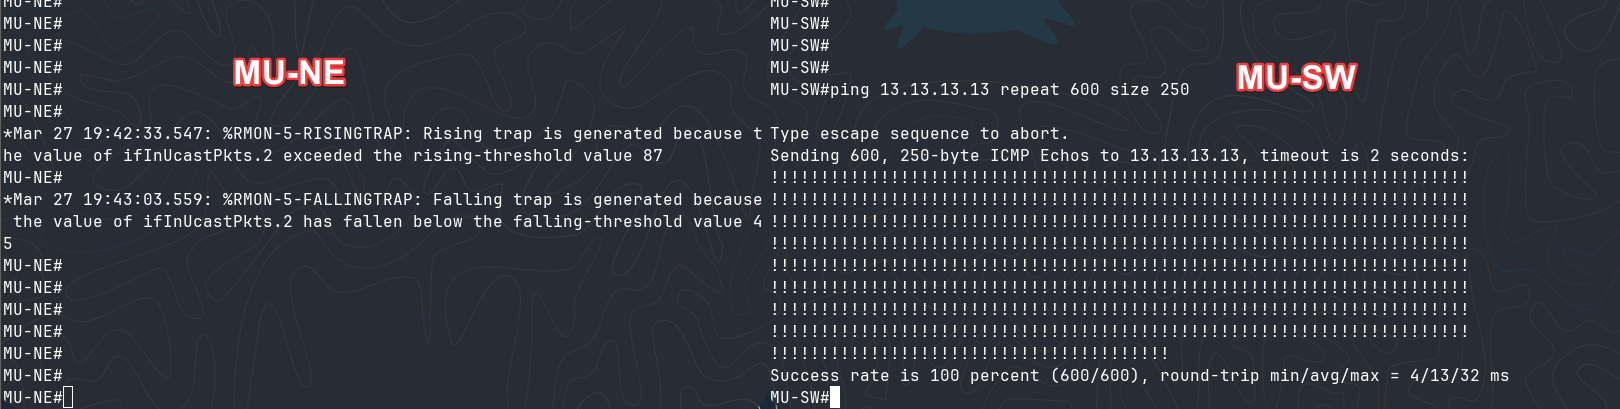
\includegraphics[width=\textwidth]{src/alarm1.png}
    \caption{Comprobación de la alarma 1}
\end{figure}

También observamos los eventLogs y demás desde MIB Browser.

\begin{figure}[h]
    \centering
    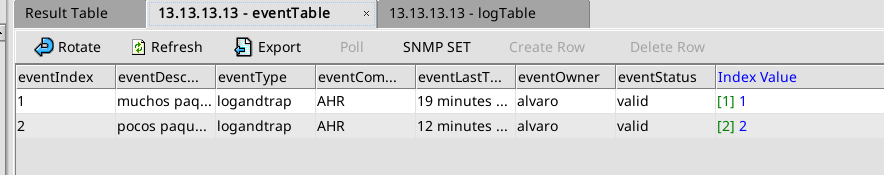
\includegraphics[width=\textwidth]{src/eventsmibs.png}
    \caption{Eventos configurados, aparecen en el MIB Browser}
\end{figure}
\begin{figure}[h]
    \centering
    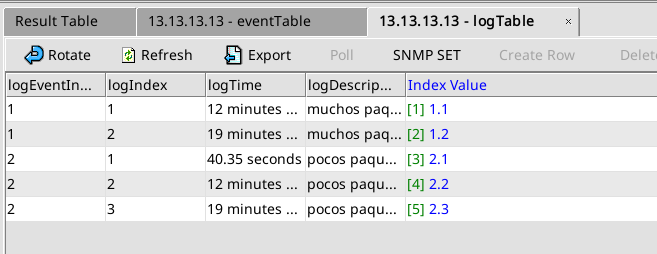
\includegraphics[width=\textwidth]{src/eventlogsmibs.png}
    \caption{Logs de eventos, saltan en el MIB Browser}
\end{figure}

\newpage

\subsection{Alarma 2: MU-NW}

Para la segunda alarma, se elegirá analizar cuando se realicen conexiones de SNMP erróneas. De esta forma, en apartados posteriores como el de Cacti, que necesitan de estas conexiones, se podrá monitorizar si se están realizando conexiones erróneas. El objeto que se usará será \texttt{snmpInBadCommunityNames}, que indicará si se ha hecho una petición de SNMP con una comunidad incorrecta, en este caso la úica comunidad configurada es AHR.

Se añade al router \texttt{MU-NW} lo siguiente:

\begin{tcolorbox}[
    boxrule=0pt,
    title=Configuración RMON Alarma 2 en MU-SW,
]
    \begin{lstlisting}[gobble=6]
         - rmon alarm 2 snmpInBadCommunityNames.0 60 absolute
         rising-threshold 1 3 falling-threshold 0 4 owner AHR
         - rmon event 3 log trap acs description ``Intento SNMP con
         comunidad incorrecta detectado'' owner AHR
         - rmon event 4 log trap acs description ``Contador SNMP bad
         community bajo (<=0)'' owner AHR
    \end{lstlisting}
\end{tcolorbox}


Se puede comprobar la configuración completa, y en todo caso la alarma se tendrá el "trigger" cuando se intente conectar con una comunidad incorrecta. Por ejemplo, con \texttt{
[lab@fedora \textasciitilde ]\$ snmpget -v2c -c HOLA 172.18.0.202 sysDescr.0}, nos saltará la alarma porque no existe la comunidad \texttt{HOLA}.


\section{\texorpdfstring{Generación de tráfico Cisco IP SLA}{Generacion de trafico Cisco IP SLA} \label{section:Generacion de trafico Cisco IP SLA}}

En este ejercicio se configurarán las IP SLA para, de alguna forma, simular tráfico constante en nuestra red, de esta forma se podrá monitorizar en los apartados siguientes.

Prácticamente sólo hay una forma de hacer este apartado, debido a que los comandos son los que proporciona cisco en su router, por lo que se ha seguido con los comandos de \texttt{ip sla} para los tres apartados. Configuraremos un cada uno con una id distinta, siendo \texttt{ip sla <id>}, y luego la acción, que en nuestro caso se piden tres, que serán:

\begin{tcolorbox}[
    boxrule=0pt,
    title=Formato de ip sla dependiendo de la acción ,
]
    \begin{lstlisting}[gobble=6]
        - icmp-echo <ip>
        - tcp-connect <ip> <port>
        - http get <url>
        - frequency, tos...
        - ip sla schedule <id> life forever start-time now
    \end{lstlisting}
\end{tcolorbox}

Las configuraciones al completo, están en el archivo \texttt{ipsla.yml}.

Interceptamos el tráfico con Wireshark para comprobar que se está generando correctamente, en las interfaces correspondientes:

\begin{figure}[h]
    \centering
    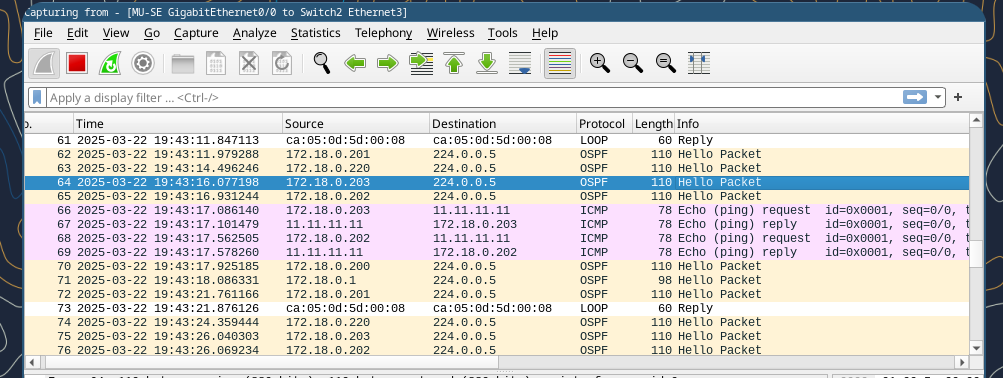
\includegraphics[width=\textwidth]{src/icmp1.png}
    \caption{Tráfico en wireshark 1}
\end{figure}
\begin{figure}[h]
    \centering
    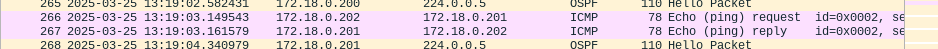
\includegraphics[width=\textwidth]{src/icmp2.png}
    \caption{Tráfico en wireshark 2}
\end{figure}
\begin{figure}[h]
    \centering
    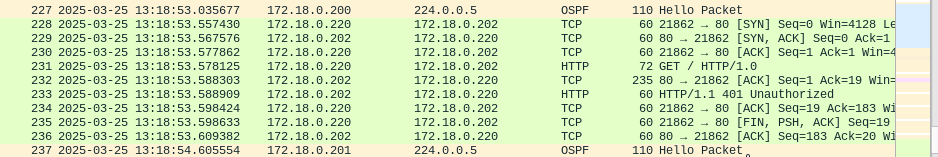
\includegraphics[width=\textwidth]{src/http1.png}
    \caption{Tráfico en wireshark 3}
\end{figure}


Con este tráfico se podrá monitorizar de forma más sencilla en los siguientes apartados.


\clearpage

\section{Monitorización con Cacti}

Para la monitorización con Cacti, se seguirá la práctica que se dió en clase, y se añadirán todos los routers y dispositivos disponibles para mostrar finalmente las gráficas del tráfico. Lo primero será iniciar Cacti con portainer y \textbf{nginx} para el proxy inverso que nos permite acceder a la interfaz de la webapp.

Tras añadir el site, tree y configuración inicial, el cual no cambia con respecto a la práctica a excepción de los campos de nombres, se añadirán los cinco routers, este es el campo a rellenar:

\begin{figure}[h]
    \centering
    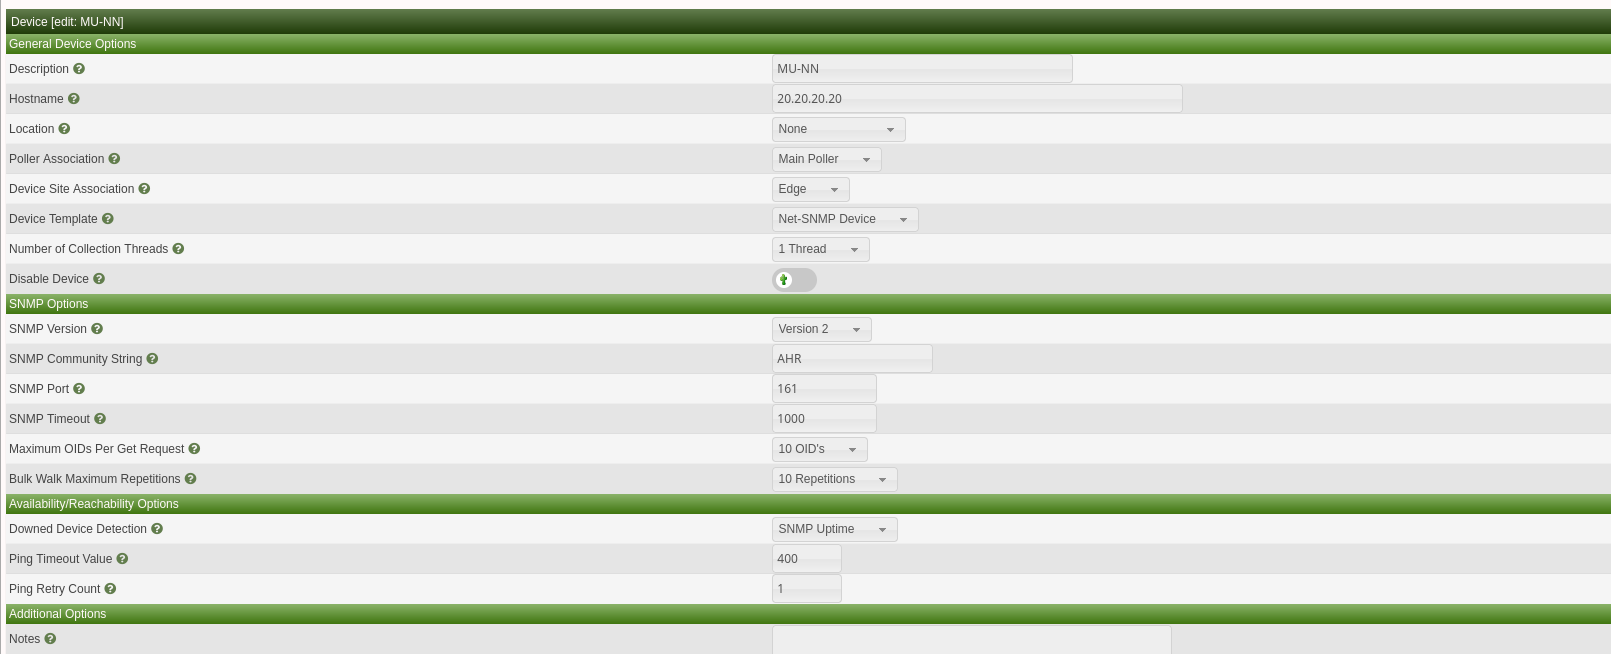
\includegraphics[width=\textwidth]{src/adddevices.png}
    \caption{Añadir dispositivo en Cacti}
\end{figure}

Una vez se haya añadido todos, importante añadir la comunidad de SNMP, se comprueba que están todos añadidos y en estado \textbf{up}.

\begin{figure}[h]
    \centering
    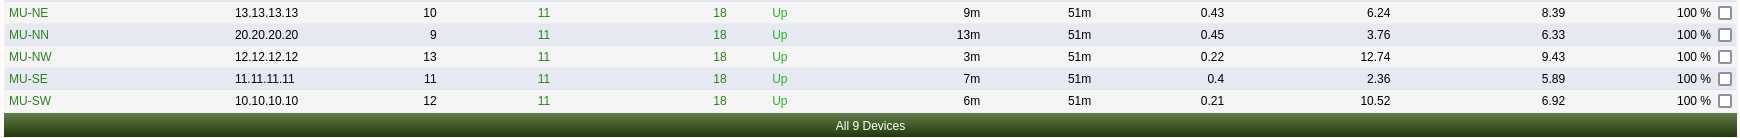
\includegraphics[width=\textwidth]{src/devices.png}
    \caption{Dispositivos añadidos en Cacti}
\end{figure}

tras esto, se crea el \textbf{Arbol} con las etiquetas correspondientes, cuya forma será:

\begin{figure}[h]
    \centering
    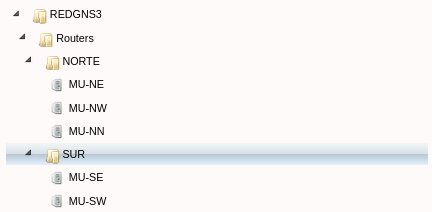
\includegraphics[width=\textwidth]{src/cactree.png}
    \caption{Árbol de dispositivos en Cacti}
\end{figure}


Se irá dispositivo por dispositivo añadiendo el \textbf{Graph} necesario. En nuestro caso, se usará el Traffic BW de \textbf{Gi0/0}. Una vez estén todas las gráficas añadidas, lo comprobamos para nuestro árbol creado:

\begin{figure}[h]
    \centering
    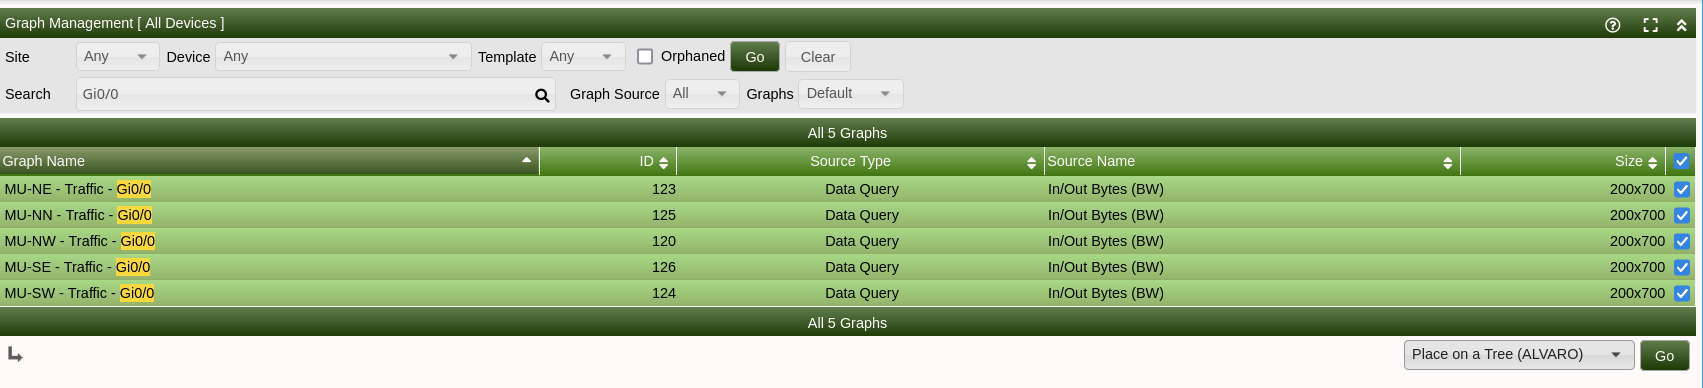
\includegraphics[width=\textwidth]{src/cactigraphs.png}
    \caption{Árbol de dispositivos en Cacti}
\end{figure}

Finalmente, recogemos las gráficas importantes en la misma zona:

\begin{figure}[h]
    \centering
    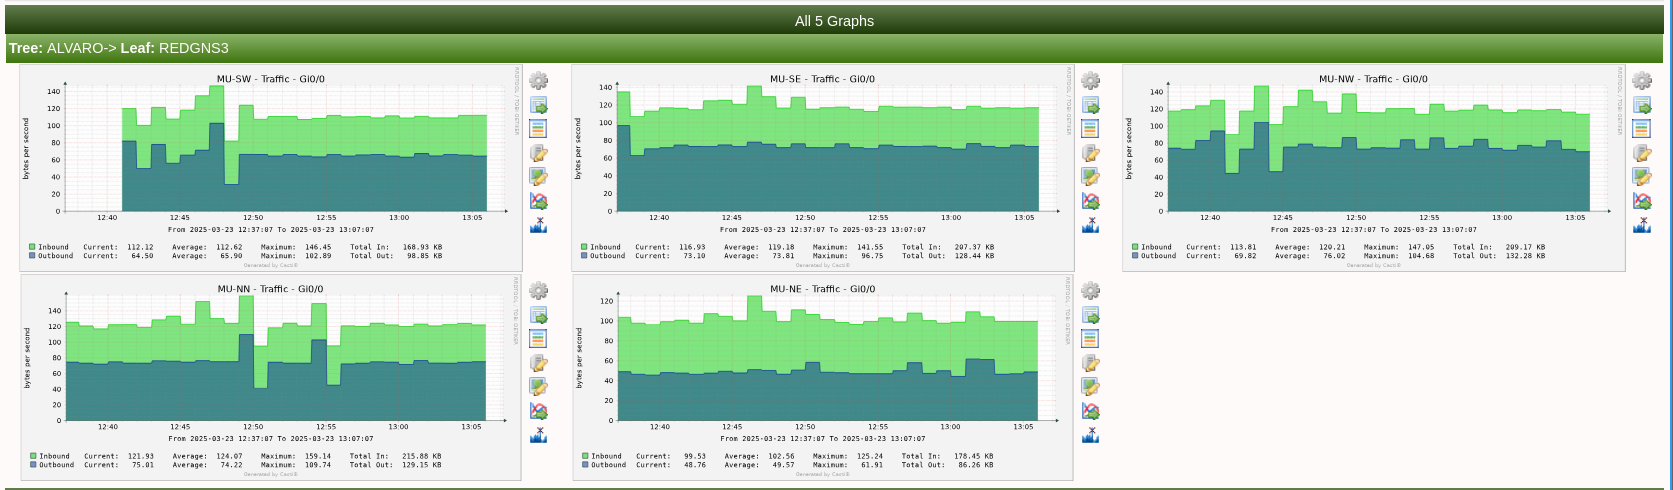
\includegraphics[width=\textwidth]{src/finalgraphs.png}
    \caption{Gráficas de Cacti}
\end{figure}



\section{Monitorización de flujos de tráfico}
\subsection{Netflow}

Este ejercicio recoge la monitorización planteada con \texttt{Netflow}, en las interfaces que planteamos el \texttt{ip sla} del  \textbf{\hyperref[section:Generacion de trafico Cisco IP SLA]{ejercicio 5}.}

Se empezará por activar netflow en todos los routers, el archivo \texttt{netflow.yml} tendrá esta forma para cada router:


\begin{tcolorbox}[
    boxrule=0pt,
    title=Formato de configuración netflow.yml,
]
    \begin{lstlisting}[gobble=6]
          - ip cef
          - int g0/0
          - ip flow ingress
          - ip flow egress
          - ip flow-export destination 172.18.0.1 2075
          - ip flow-export destination 172.18.0.1 2055
          - ip flow-export version 5
    \end{lstlisting}
\end{tcolorbox}

Se puede ver que está el puerto configurado de 2055 y 2075, por el momento solo nos interesa el 2075, más adelante, para el \texttt{OpenObserve}, usaremos el otro puerto.

Ahora comprobaremos la cache:

\begin{figure}[h]
    \centering
    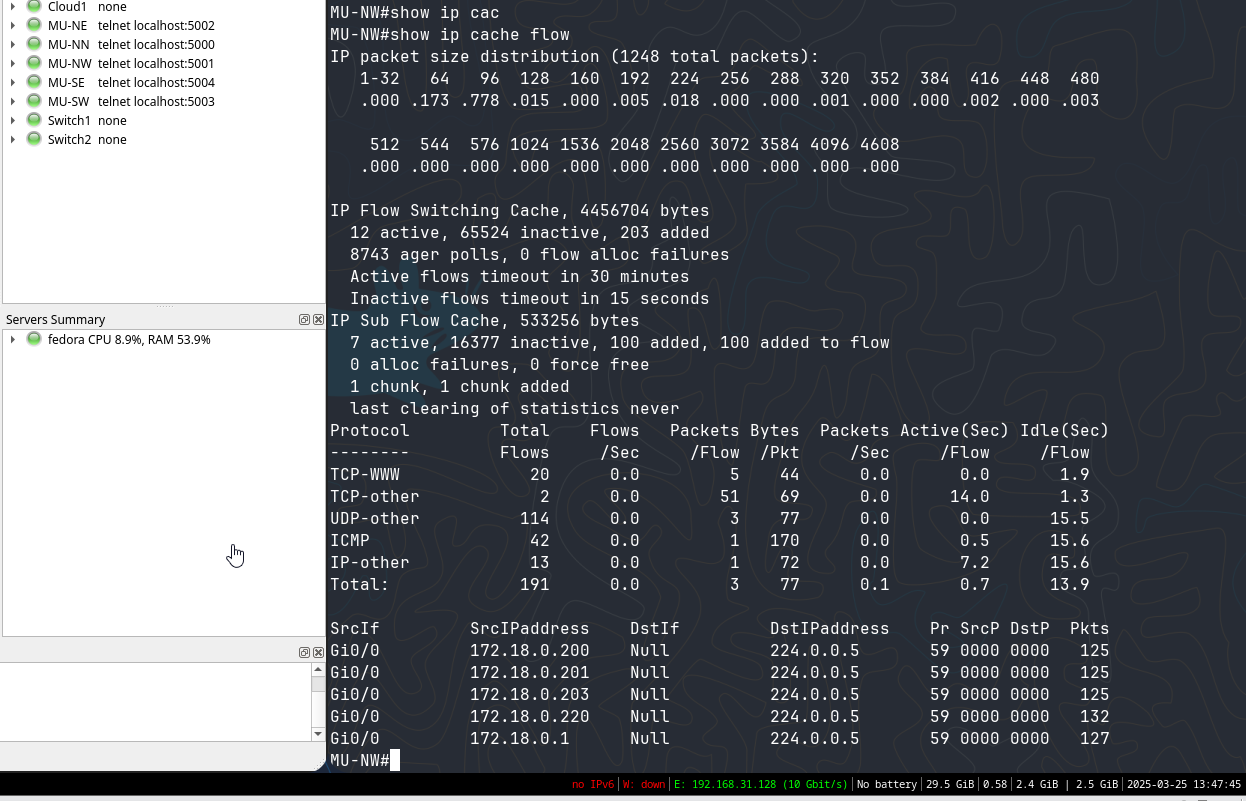
\includegraphics[width=\textwidth]{src/cacheflow.png}
    \caption{Cache de netflow}
\end{figure}


Para configurar el colector, se seguirá la práctica que se dio en clase, teniendo en cuenta lo que significa cada parte del comando y la ruta a guardar. El comando usado se puede observar en la captura:

\begin{figure}[h]
    \centering
    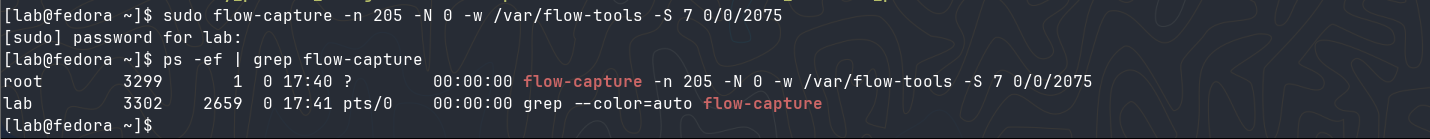
\includegraphics[width=\textwidth]{src/comandoflow.png}
    \caption{Comando de configuración del colector}
\end{figure}

Finalmente, como nuestro colector está configurado para guardar cada 7 minutos, veremos un archivo cada 7, y podemos imprimir el flow-print de un archivo para ver lo que ha generad en 7 minutos. En la captura se puede observar tanto el comando con el print, como el nombre y la fecha en la que se crean los archivos de tráfico

\begin{figure}[h]
    \centering
    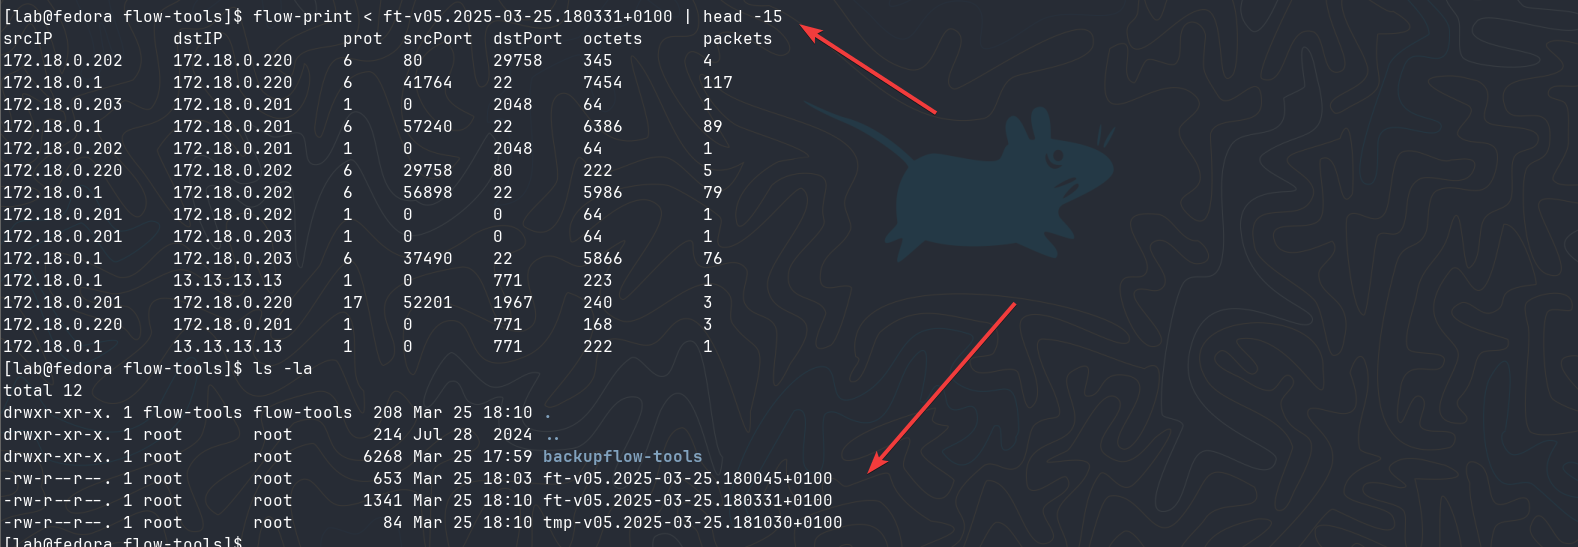
\includegraphics[width=\textwidth]{src/flowprint.png}
    \caption{Comando de print de netflow}
\end{figure}
\begin{figure}[h]
    \centering
    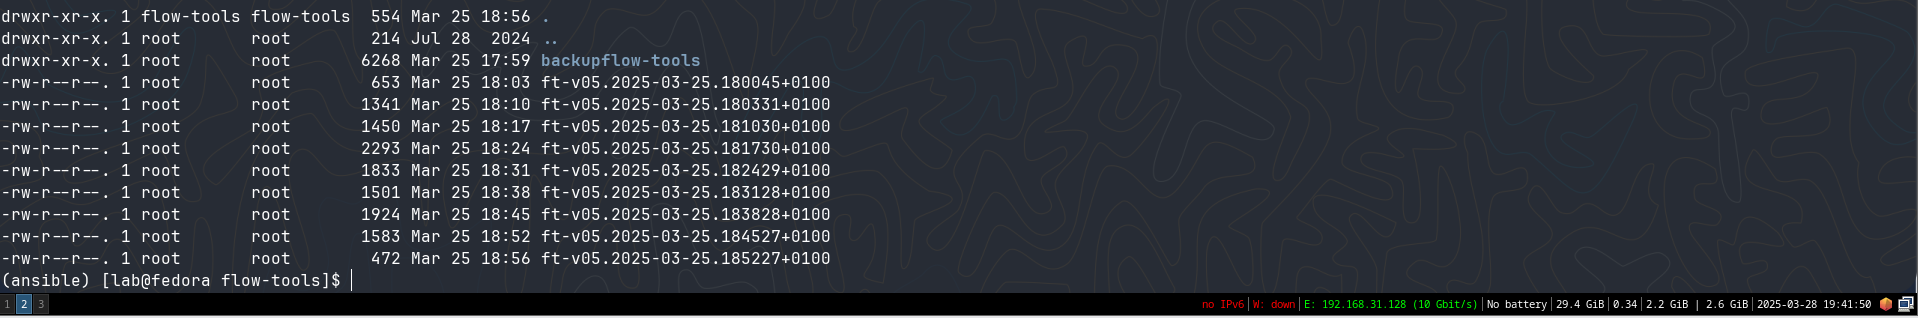
\includegraphics[width=\textwidth]{src/lsflow.png}
    \caption{Archivos de flujo}
\end{figure}

\newpage 

\subsection{OpenObserve}

Para esta sección, al tener ya todo configurado y el puerto 2055 también está añadido como destino, se iniciará open OpenObserve mediante \textbf{portainer}, junto a su añadido de goflow. 

Filtraremos en la tabla de flujos para ver el timestamp, protocolo, dirección origen, dirección destino, y siguiente salto, al igual que el histograma que estará en la parte superior de la captura.


\begin{figure}[h]
    \centering
    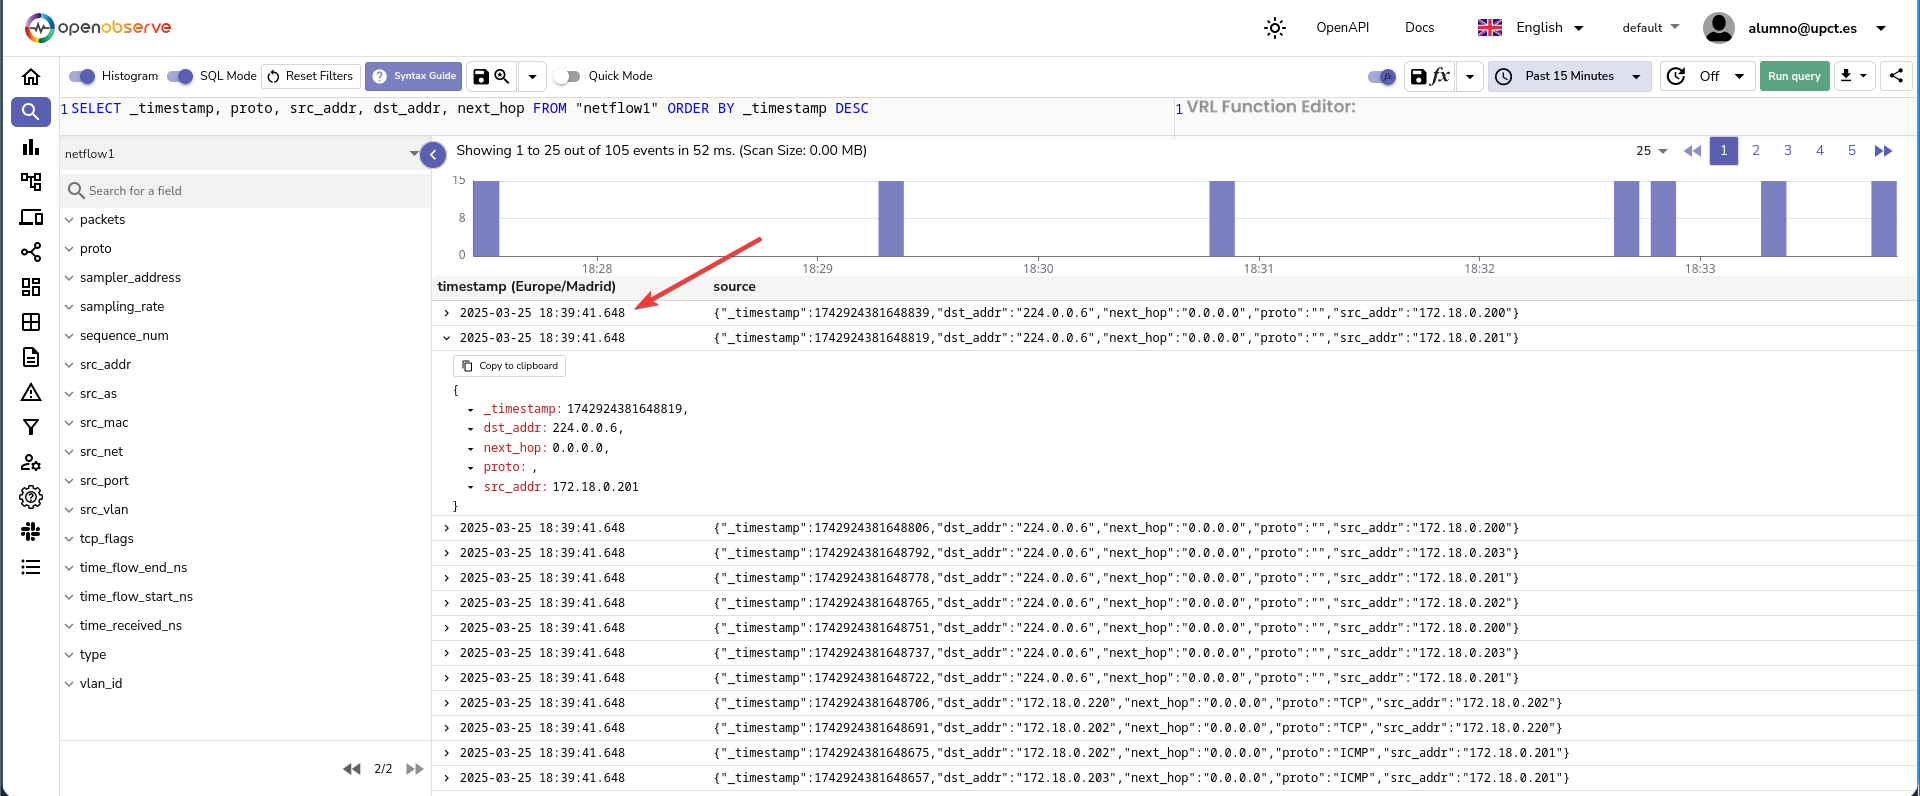
\includegraphics[width=\textwidth]{src/flujos.png}
    \caption{Tabla de flujos openobserve}
\end{figure}

Para la parte final, se hará una captura del dashboard \texttt{Network Activity, } el cual se ha añadido mediante \texttt{json} desde el github de \texttt{OpenObserve}. 

\begin{figure}[h]
    \centering
    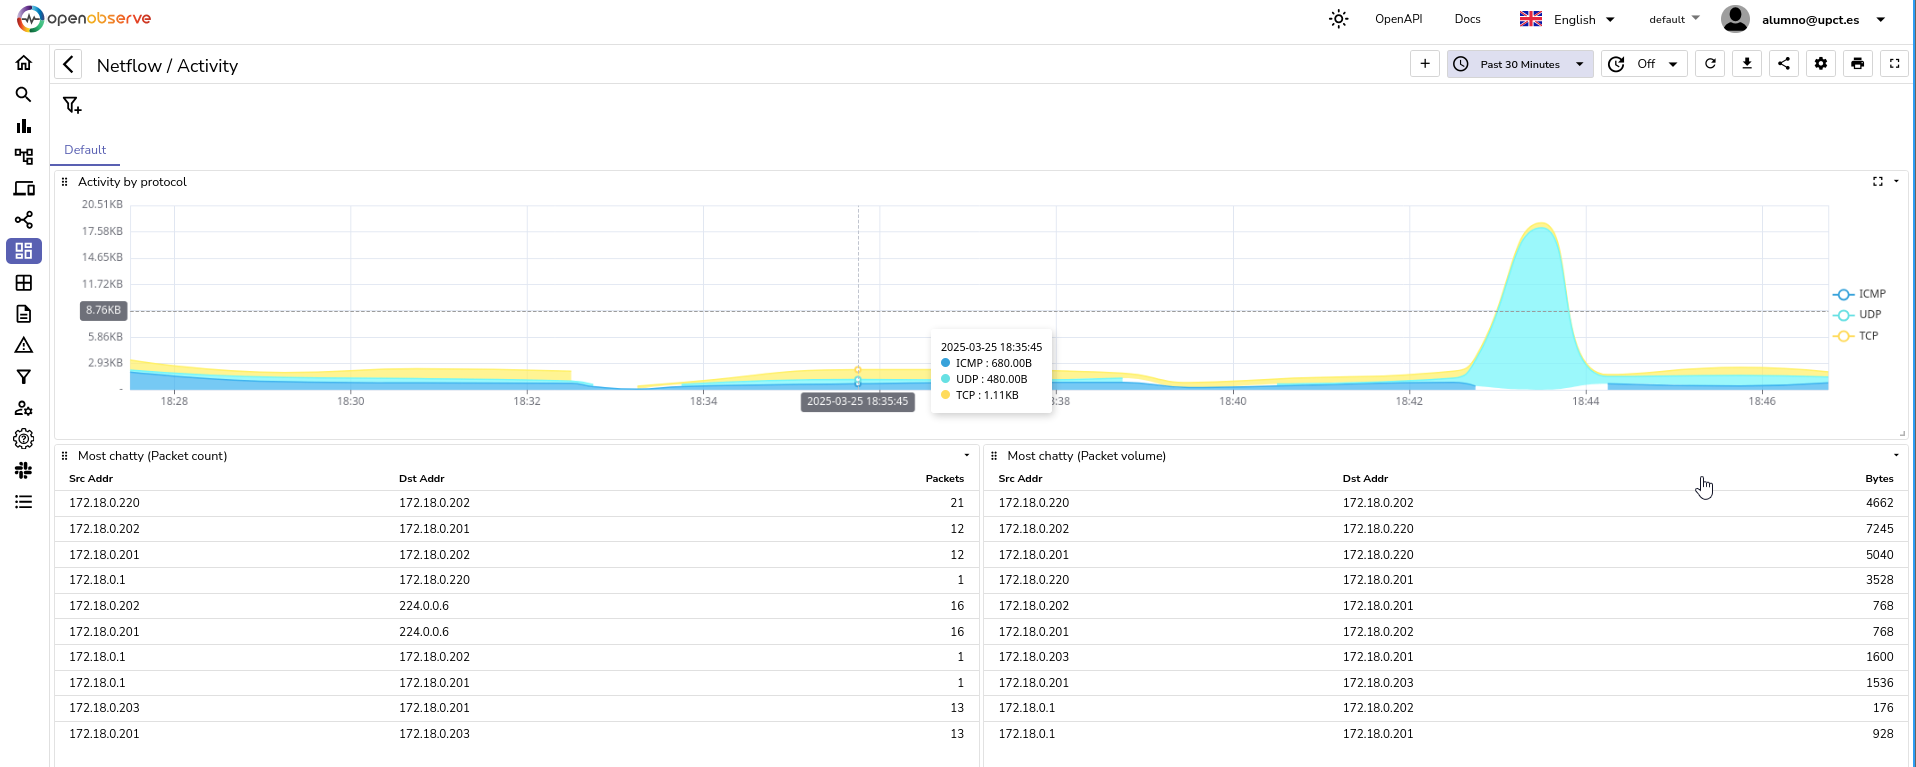
\includegraphics[width=\textwidth]{src/openobs1.png}
    \caption{Gráfico de openobserve con udp}
\end{figure}

Como se puede ver, hay un pico enorme de UDP, posiblemente de algunas configuracones o peticionies que se hayan hecho a los routers fuera del tráfico SLA que hemos configurado, si filtramos por el tráfico que no es UDP, se puede ver un tráfico más constante:

\begin{figure}[h]
    \centering
    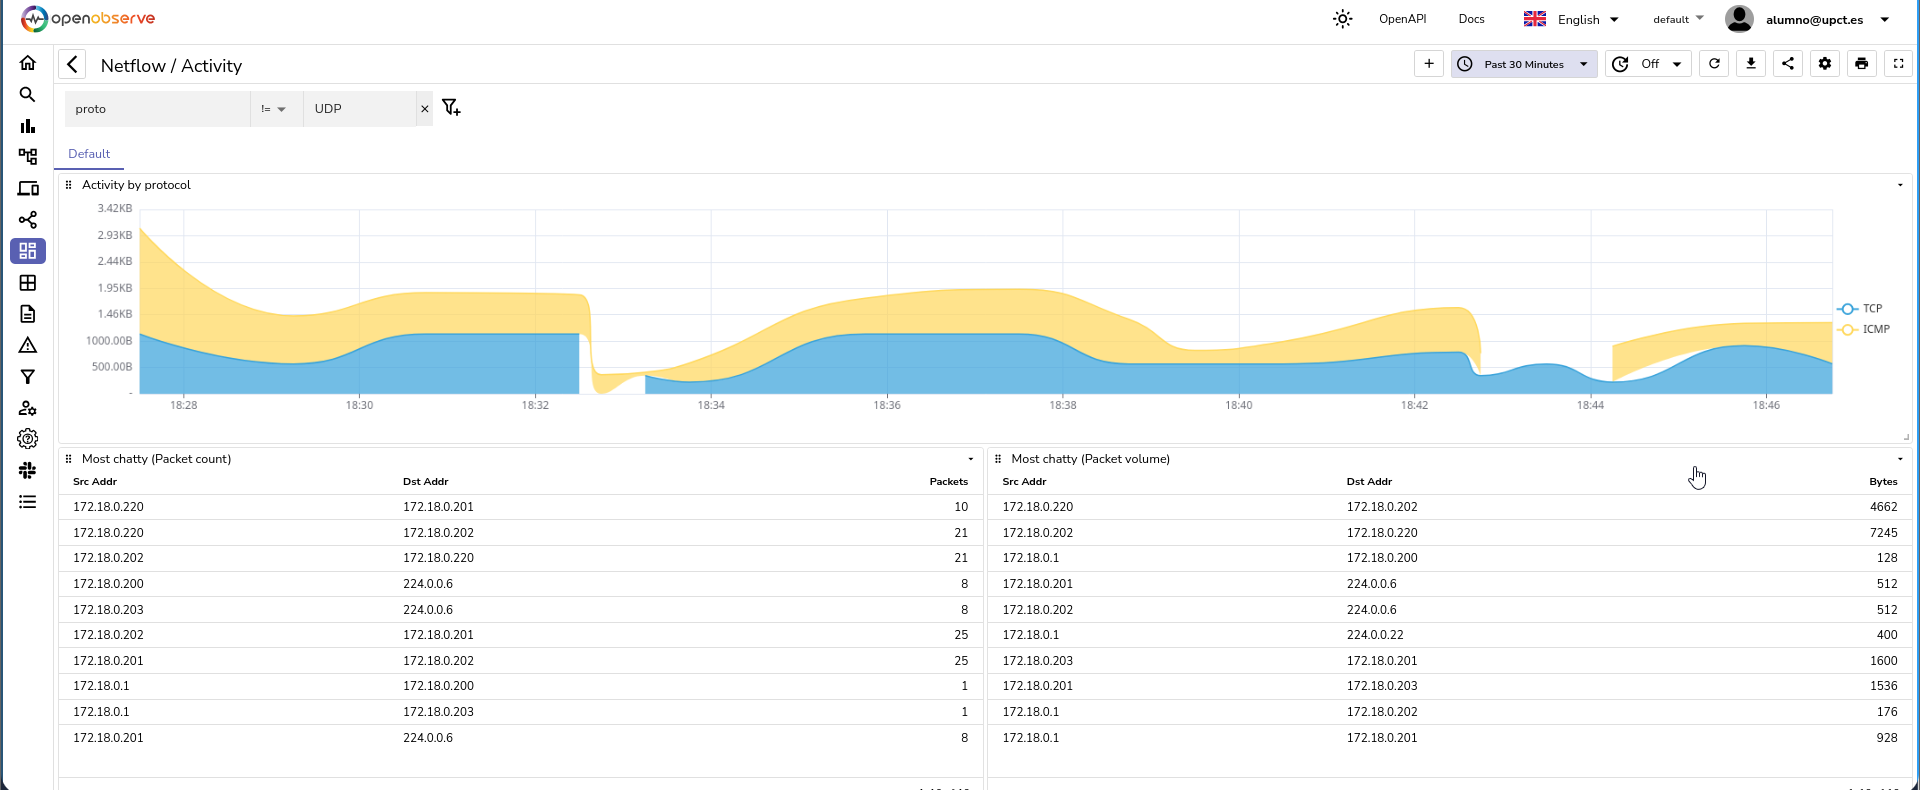
\includegraphics[width=\textwidth]{src/openobs2.png}
    \caption{Gráfico de openobserve sin udp}
\end{figure}


\end{document}